\documentclass[../p052main.tex]{subfiles}
\graphicspath{{\subfix{../figures/}}}

\begin{document}

\chapter{Applications}
\section{Band Structure of Solids}
As an application of what we've done so far, we'll do a first-principles investigation into some properties of solids.
Consider a block of metal; the potential in this metal is generally periodic, with asymptotes to negative infinity at each nucleus.
We might simplify things by approximating each asymptote as a finite square well, but for our purposes it will do to use a series of upward delta spikes at the midpoints between atoms:
\[ \frac{2mV(x)}{\hbar^2} = \frac{\alpha}{a} \sum_{n=1}^{N} \delta(x - na), \]
where $a$ is the separation between the spikes and $\alpha$ is the ``strength'' of each spike.
We'll build in two more elements of periodicity.
\begin{itemize}
    \item The wave function's corresponding probability density function must be periodic with period $a$.
    Mathematically, $| \psi(x + a)|^2 = |\psi(x)|^2$, and we get $\psi(x+a) = e^{i\theta} \psi(x)$.
    This is called the Bloch ansatz.

    \item If we imagine our one-dimensional lattice to be a closed loop then the wave function itself must be single-valued and so must be periodic with period $Na$, where $N$ is the number of atoms in the metal.
    Thus $\psi(x + Na) = \psi(x)$
\end{itemize}
Combining these, we find that $\psi(x + Na) = e^{iN\theta} \psi(x) = \psi(x)$ and $e^{iN\theta} = 1$.
Thus $\theta = 2 \pi r / N$, where $r$ is an integer falling between $0$ and $N-1$.
Now, using the time-independent Schrödinger equation we find that, in each region between spikes, we have
\[ \psi_n(x) = A_n \sin \big( k(x - na) \big) + B_n \cos \big( k(x - na) \big), \quad (n-1)a < x < na. \]
Notice that by the Bloch ansatz we have $A_{n+1} = e^{i\theta} A_n$ and $B_{n+1} = e^{i\theta} B_n$, so we really only have three unknowns: $A_1$, $B_1$, and $k$.
To restrict them, we begin by applying the continuity boundary condition $\psi_n(na) = \psi_{n+1}(na)$ to get
\[ B_n = B_n e^{i\theta} \cos ka - A_n e^{i\theta} \sin ka. \]
Also, $\psi$ is not differentiable, but it does satisfy $\left( d\psi / dx \right)_{na^+} - \left( d\psi / dx \right)_{na^-} = (\alpha / a) \psi_n(na)$.
This gives
\[ \frac{\alpha}{ka} B_n = A_n e^{i\theta} \cos ka + B_n e^{i\theta} \sin ka - A_n. \]
If we rewrite both of these equations such that all $A_n$ are on the left and all $B_n$ on the right and then divide, we end up with
\[ \cos \theta = \cos ka + \frac{\alpha}{2ka} \sin ka, \quad \theta = \frac{2\pi r}{N}. \]
Solving this equation for $k = \sqrt{2mE} / \hbar$ gives the allowed energies for the system.
This cannot be done analytically, but we can glean some information using the below plot of the equation's right-hand side.

Due to the range restriction on $\cos \theta$, the only allowed $ka$ are those for which the curve is bound by $[-1, 1]$.
The energies corresponding to the allowed $ka$ are plotted on the right.
We see a structure of widening bands and narrowing gaps take form.
Note that this is not an artifact of our delta potential model---if we stuck with the more realistic asymptote model we'd see something similar.

\section{Electrical Properties of Solids}
As it turns out, this is the most fundamental characteristic of conductors and insulators as groups!
A material is a conductor if its Fermi energy falls inside of a band; in this case there are energies available for ``accelerated'' electrons to fill upon being influenced by an electric field.
Otherwise the material is an insulator or a semiconductor, depending on how large the gap to the next band up is.
(Also, solids with one valence electron per atom are conductors since, due to spin degeneracy, there is certainly a band that is not full.
We cannot make a definite statement about solids with two valence electrons per atom.)

\begin{center}
    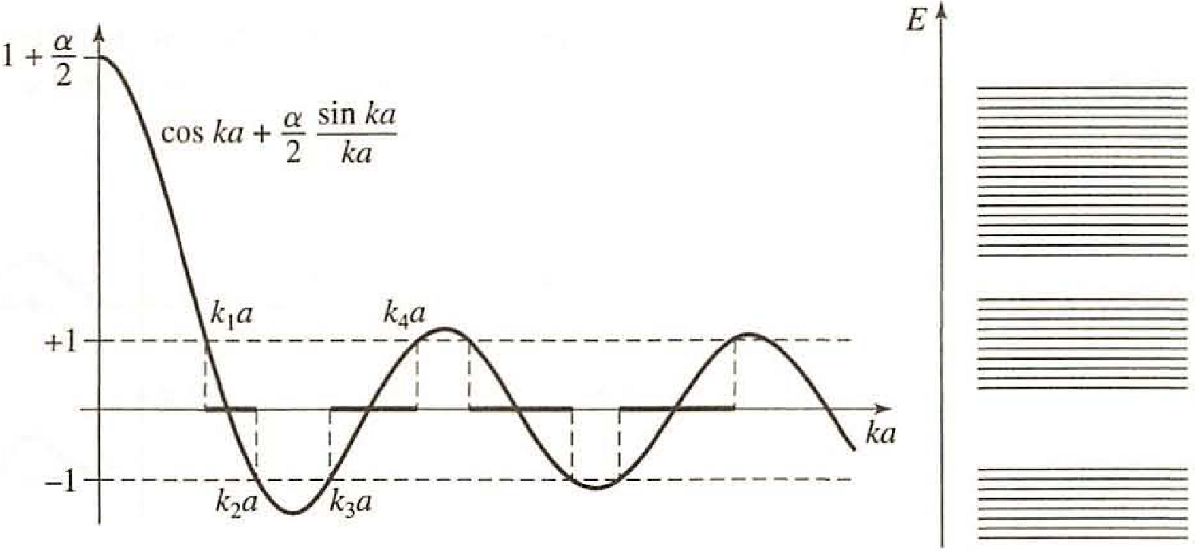
\includegraphics[width=0.85\textwidth]{bandGapSols.png}
\end{center}

% \section{Electrical Properties of Solids}
% As it turns out, this is the most fundamental characteristic of conductors and insulators as groups!
% A material is a conductor if its Fermi energy falls inside of a band; in this case there are energies available for ``accelerated'' electrons to fill upon being influenced by an electric field.
% Otherwise the material is an insulator or a semiconductor, depending on how large the gap to the next band up is.
% (Also, solids with one valence electron per atom are conductors since, due to spin degeneracy, there is certainly a band that is not full.
% We cannot make a definite statement about solids with two valence electrons per atom.)

Sometimes the highest-allowed band is called the valence band, and the band with the next energy up is called the conducting band.
In conductors these are the same, and we call it the metallic band.
The distance from the Fermi energy to the top of the metallic band is called the work function.

Suppose we bring two metals into close proximity to one other, so there's a very small potential barrier between them.
The metals' work functions are related by $W_a < W_b$, so the Fermi energy of metal $a$ is greater than that of metal $b$.
Electrons in $a$ can thus tunnel to the lower energies in $b$, giving $a$ a positive charge and $b$ a negative charge.
The potential energy of an electron in $a$ falls, and that of an electron in $b$ rises.
This has the overall effect of shifting the metals' Fermi energies until an equilibrium is reached, at which point a contact potential
\[ \phi_\textrm{contact} = \frac{W_b - W_a}{q_e} \]
exists between the two metals.

For insulators and semiconductors, at $T = 0 \textrm{ K}$ the valence band is completely filled and the conducting band is empty.
Define $E=0$ to be the top of the valence band, and $E_g$ the gap between the bands.
At a given temperature, we'd like to use the Fermi-Dirac distribution to determine the probability of occupation for a state at the bottom of the conducting band, but this requires knowing the chemical potential $\mu$.

At temperature $T$, the number of atoms excited to the conduction band and holes in the valence band are respectively given by
\[ \frac{1}{e^{(E_g - \mu) / k_BT} + 1} D(E_g) \,dE, \qquad \left( 1 - \frac{1}{e^{(-\mu) / k_BT} + 1} \right) D(0) \,dE. \]
The number of conducting electrons is equal to the number of valence holes, so
\[ \frac{1}{e^{(E_g - \mu) / k_BT} + 1} D(E_g) \,dE = \left( 1 - \frac{1}{e^{(-\mu) / k_BT} + 1} \right) D(0) \,dE. \]
Assuming $D(0) = D(E_g)$, solving gives $\mu = E_g / 2$, right in the middle of the band gap.
This quantity is also called the Fermi level, a generalization of the Fermi energy that denotes the energy of a quantum state with 50\% probability of being filled at a temperature $T$.
Note that if $E_g \gg k_BT$ we get $n_\textrm{FD}(E_g) \simeq e^{-E_g / 2k_BT}$, and we see that there are correspondingly few holes in the valence band.

We can create a couple of particularly important kinds of semiconductors through a process called doping.
Take a block of silicon for example; on its own this silicon is insular, but we can replace an extremely small fraction of silicon atoms with other atoms with different numbers of valence electrons.
The idea is to keep the same band structure, but to change the number of electrons inhabiting that structure.
\begin{itemize}
    \item If we dope with gallium, which has one fewer valence electron than silicon, then there is a deficit of electrons and we get some holes at the top of the valence band.
    This creates a p-type semiconductor, and the Fermi level is a little under the halfway point.

    \item If we dope with arsenic, which has one more valence electron than silicon, then we get some extra electrons at the bottom of the conducting band.
    This creates an n-type semiconductor, and the Fermi level is a little above the halfway point.
\end{itemize}
We can put these two semiconductors side by side in very close proximity to create a p-n junction.
Just as we saw with metals, electrons from the n side move to lower energy levels on the p side until the two Fermi levels align.
This creates negative and positive charges on the p and n sides, respectively, and thus an electric field exists in the depletion region between the sides.

Even in equilibrium charges are still moving, just in equal amounts.
On the p side electrons are excited by thermal energy into the conduction band, where they find a downhill potential and slide onto the n side; this is called the thermal current $I_0$.
On the n side electrons are excited by thermal energy onto the p side, generating the recombination current $I_R$.

So in equilibrium we have $I_0 = I_R$.
But if we apply an external potential $\phi$ to the junction, the recombination current must change so that a nonzero net current may flow.
Depending on whether it increases or decreases, we have one of $I_R = I_0 e^{\pm |\phi| q_e / k_B T}$.
Using $I = I_R - I_0$, we can express the net current in terms of $I_0$.
This is the foundation of technologies like LDEs, photovoltaic cells, and transistors!

We'll look at one last kind of material: superconductors.
The important property here is the resistivity $\rho$, which is related to resistance by $R = \rho (L / A)$ where $L$ is a tiny length of a cross section $A$.
In any material, the electrons are scattering about due to interactions with vibrating nuclei, and this scattering gets less prevalent as temperature decreases.
In particular,
\[ \rho = \frac{m}{nc^2} \frac{1}{\tau}, \]
where $1 / \tau$ is the temperature-dependent scattering rate.
For most materials the resistance simply diminishes to some $R_0$.
However, experiments show that there are some for which there is a critical temperature $T_c$ after which the resistance drops to literal zero.
This is what characterizes a superconductor!

The idea here is that pairs of electrons can come together to act like a boson.
When two electrons in a lattice have opposite momenta, they are attracted each other via distortions in the lattice; these distortions are significant since the repulsion between two electrons is much smaller in a lattice than it is in a vacuum.
In $k$-space, we interpret these as electrons with opposite $\mbf{k}$ and opposite spin being attracted and forming a bound state (with a lower energy) relative to the Fermi energy.
This is what we call a Cooper pair.

If $\mbf{R}_\textrm{CM}$ and $\mbf{k}_\textrm{CM}$ are the center of mass and average $k$-space vectors, then it turns out that the wave function looks like
\[ \Psi_\textrm{pair}(1,2) = e^{i (\mbf{k}_\textrm{CM} \cdot \mbf{R}_\textrm{CM})} \Psi(\mbf{\mbf{r}_1 - \mbf{r}_2}) \chi(1,2). \]
Since the electrons are fermions we need an overall antisymmetric state, so we take
\[ \chi(1,2) = \frac{1}{\sqrt{2}} \big[ \chi_+(1)\chi_-(2) - \chi_-(1) \chi_+(2) \big]. \]
So our Cooper pair behaves like a boson, and the Pauli exclusion principle no longer applies!
All Cooper pairs in existence can fall into the same ground state.
This is the superconducting state.

There are three hallmarks of such a state.
First, as we saw, it has zero resistance.
Also, a material in a superconducting state is a perfect diamagnet; specifically, it has magnetic susceptibility $\chi_m = -1$.
Finally, the magnetic flux through a loop of superconducting is quantized in integer multiples of $h / 2q_e$---this is a direct consequence of requiring a single-valued wave function.

\section{Nuclei and Binding Energy}
Let's begin again by loosely discussing the structure of an atom.
We know, by now, that on scales these small it doesn't really make sense to discuss definite sizes, but we can at least pin down general spheres of influence---the characteristic radius of an atom is around $R_\textrm{atom} \sim 1 \textrm{ \AA} = 10^{-10} \textrm{ m}$, and that of a nucleus is $R \sim 1 \textrm{ fm} = 10^{-15} \textrm{ m}$.
The proton and neutron (together, nucleon) masses are on the order of $10^{27} \textrm{ kg}$ and only differ in their fourth digits, so we approximate $m_n \simeq m_p$; the electron mass is on the order of $10^{-30} \textrm{ kg}$.
Note that free neutrons are unstable and decay according to \ch{n -> p^+ + e^- + $\overline{\nu}$_e} with half-life $(610 \pm 1) \text{ s}$.
(The $\overline{\nu}_e$ is called an electron antineutrino; more on that later.)

Some notation will be useful.
The symbol \ch{_{$Z$}^{$A$}X} has three parts: the element symbol X, the atomic number $Z$, and the mass number $A$.
(With $N$ neutrons we have $A = Z + N$.)
As shorthand, we'll often also write
\begin{center}
    \ch{^11H \;=\; p}, \quad \ch{^21H \;=\; n}, \quad \ch{^31H \;=\; t}, \quad \ch{^42He \;=\; $\alpha$}.
\end{center}
Note that the mass number is always an integer, while on the periodic table we usually see decimals.
This is because the periodic table values are weighted averages over all stable isotopes---in hydrogen, for example, we'd include p and d but not t.
The stabilities of different isotopes are visualized very nicely with $N$ and $Z$ on the horizontal and vertical axes, respectively; when we color each cell according to its half-life we see a roughly linear correlation between $N$ and $Z$ whose slope is a little less than 1.
This linearity subtly breaks down at higher $N$, reflecting how we need more neutrons to keep the nuclei together as we add more protons.

It's possible to roughly determine the size of a nucleus as a function of its mass number $A$.
We can't do this using light without using crazy high-energy gamma rays, so instead some clever electron scattering experiments have been done to probe nuclear charge distributions.
It turns out that these distributions are roughly constant in the interior, so if we define $R$ as the radius at which the charge starts dropping off we get $R \simeq r_0 A^{1 / 3}$ with $r_0 = 1.2 \textrm{ fm}$.
This gives the volume $V = V_0 A$, where $V_0 = 7.2 \textrm{ fm}^3$ is the nucleon volume based on its characteristic radius $r_0$.
It follows that nuclear matter has a mass density on the order of $10^{17} \textrm{ kg/m}^3$---huge!

We could do a similar thing with neutron scattering in order to probe nucleon density rather than charge density.
Assuming each neutron is a point mass gives the neutron-nucleus cross section $\sigma = \pi R^2 = \pi r_0^2 A^{2 / 3}$.
(These cross sections are usually expressed in terms of barns, where $1 \textrm{ barn} = 1 \textrm{ b} = 10^{-28} \textrm{ m}^2$.)
This guess is unsurprisingly wrong, but it is on the correct order of magnitude.
We could get a more accurate depiction of these interactions by relaxing the assumption that a neutron is a point particle and by using its $\lambda_\textrm{dB}$.

Now, the stability of an isotope is determined by its binding energy, which is the difference between the mass energy associated with a nucleus versus that associated with the sum of its individual parts.
Mathematically,
\[ E_B = \left( Z m_p c^2 + (A - Z) m_n c^2 \right) - m_\textrm{nuc} c^2. \]
The higher the $E_B$, the more stable a nucleus is because it takes more energy to ``free'' the nucleons.
So it will be productive to determine how, exactly, the binding energy is set.

We'll building up to the semi-empirical formula
\[ E_B = a_1 A - a_2 A^{2 / 3} - a_3 \frac{Z^2}{A^{1 / 3}} - a_4 \frac{(Z - A / 2)^2}{A} + \frac{a_5}{A^{1 / 2}} \begin{pmatrix} 1 \\ 0 \\ -1 \end{pmatrix}, \]
where the fitted coefficients follow $a_4 > a_1, a_2, a_5 > a_3$.
The first terms can be explained using the liquid drop model in which the nuclei are spherical, incompressible, and constant-density in both mass and charge.
Every nucleon interacts via a short-range attractive nuclear force with its nearest neighbors, and all protons interact with each other via the long-range Coulomb force.
\begin{itemize}
    \item[1.] Volume term.
    Due to nearest-neighbor interactions we have a positive $E_1 = A n_\textrm{NN} \propto A$

    \item[2.] Surface term.
    We've over-counted since surface nucleons have less neighbors than inner ones.
    Since the nuclear surface area is proportional to $A^{2 / 3}$ we subtract an $E_2 \propto A^{2 / 3}$.

    \item[3.] Coulomb term.
    Now we account for Coulomb repulsion.
    From E\&M we know that the energy associated with a ball of charge $Ze$ is proportional to $Z^2 / R$, so we subtract an $E_3 \propto Z^2 / A^{1 / 3}$.
\end{itemize}
Now let's switch to a different, Fermi gas model.
We'll model the strong nuclear force as a half-infinite square well, and we'll stuff protons and neutrons into that well according to the Pauli exclusion principle.
\begin{itemize}
    \item[4.] Asymmetry term.
    If we have $N$ fermions, then the total energy associated with those fermions is $E_\textrm{tot} = \frac{3}{5} N E_F$.
    Doing this for both protons and neutrons gives
    \begin{align*}
        E_\text{tot} &= \frac{3}{5} Z \frac{\hbar^2}{2m_p} \left( \frac{3\pi^2 Z}{V} \right)^{2 / 3} + \frac{3}{5} (A - Z) \frac{\hbar^2}{2m_p} \left( \frac{3\pi^2 (A - Z)}{V} \right)^{2 / 3} \\
        &= \frac{3}{5} \frac{\hbar^2}{2m_p} \left( \frac{3\pi^2}{V} \right)^{2 / 3} \left[ Z^{5 / 3} + (A - Z)^{5 / 3} \right],
    \end{align*}
    approximating $m_n \simeq m_p$.
    Thus
    \[ E_\text{tot} \propto \frac{\left[ Z^{5 / 3} + (A - Z)^{5 / 3} \right]}{A^{2 / 3}}, \]
    and minimizing this quantity with respect to $Z$ gives $Z = A / 2$.
    This gives
    \[ E_4 = E_\text{tot}(Z) - E_\text{tot}(A / 2) \propto \frac{(Z - A / 2)^2}{A}. \]
\end{itemize}
The origin of the last term is a little sketchy and has to do with symmetric and antisymmetric states.
We'll just explain how it works here.
\begin{itemize}
    \item[5.] Symmetry term.
    If the numbers of protons and neutrons are both even then the term is positive, and if they're both odd then it's negative.
    If the parities don't match then the term vanishes.
\end{itemize}
All of these together provide a very good fit for the observed binding curve, including the peak at iron-56.

\section{Radioactivity, Fusion, and Fission}
If a nucleus is unstable, it decays toward the curve of stability on the isotope table form earlier.
There are a few prominent modes by which this can happen.
\begin{itemize}
    \item $\alpha$-decay.
    The nucleus emits an $\alpha$-particle, which is our name for a \ch{^42He} nucleus.
    This causes $N \to N-2$ and $Z \to Z-2$, so we move twice down and twice left on the isotope table.
    As an example,
    \begin{center}
        \ch{^{238}92U -> ^{234}90Th + ^42He}.
    \end{center}
    
    \item $\beta^+$-decay.
    A proton decays according to \ch{p -> n + e^+ + $\nu$_e}, causing $N \to N+1$ and $Z \to Z-1$, a single down-right movement on the isotope table.
    For example,
    \begin{center}
        \ch{^{13}7N -> ^{13}6C + e^+ + $\nu$_e}.
    \end{center}
    
    \item $\beta^-$-decay.
    A neutron decays according to \ch{n -> p + e^- + $\overline \nu$_e}, causing $N \to N-1$ and $Z \to Z+1$, a single up-left movement on the table.
    For example,
    \begin{center}
        \ch{^{16}7N -> ^{16}8O + e^- + $\overline{\nu}$_e}.
    \end{center}
    
    \item p-decay.
    A proton is emitted, so $N \to N$ and $Z \to Z-1$, causing a single downward movement:
    \begin{center}
        \ch{^{11}7N -> ^{10}6C + p}.
    \end{center}

    \item n-decay.
    A neutron is emitted, so $N \to N-1$ and $Z \to Z$, causing a single leftward movement:
    \begin{center}
        \ch{^{10}3Li -> ^93Li + n}.
    \end{center}
    
    \item Spontaneous fission.
    A nucleus randomly decays into two smaller nuclei with different masses along with a few neutrons.
    One example is
    \begin{center}
        \ch{^{254}98Cf -> ^{118}46Pd + ^{132}52Te + 4 n}.
    \end{center}
\end{itemize}
By the law of radioactivity, the probability $R$ of decay per unit time is constant.
There is nothing we could possibly do to tell if a nucleus is going to decay soon.
So if we start with a number $N(t)$ of nuclei, we have
\[ N(t + dt) = N(t) - R \,dt\, N(t) \implies N(t) = N(0) e^{-t / \tau}, \]
where we $\tau$ is defined in terms of the half life: $t_{1 / 2} = \tau \ln 2$.

We can take advantage of this knowledge to determine the age of some very old objects!
If we have a substance containing trace amounts of, say, \ch{^{235}U} and \ch{^{238}U}, then if we know the half-life for each isotope and the original ratio between their amounts, then we can calculate how much time it's been sitting for.
This is one of the ways we've been able to estimate the age of the solar system.
It's also used to determine the age of dead organic material, in which case we compare the unstable \ch{^{13}C} and \ch{^{14}C} to the stable \ch{^{12}C}.

Now, it turns out that $\alpha$-decay is more common than, say, proton or neutron emission.
To see why, let's model the process using an $\alpha$-particle confined by the rest of the nucleus---it's in a deep square well, which at radius $R$ jumps up and turns into a Coulomb potential.
We determined, long ago, that the probability of the $\alpha$-particle tunneling through a potential barrier to liberate itself is given by
\[ T \simeq \exp \left[ -\frac{2 \sqrt{2m_\alpha}}{\hbar} \int \sqrt{V(r) - E_\alpha} \,dr \right] \simeq \exp \left[ -\frac{4(Z-2)}{\sqrt{E_\alpha}} \right], \]
where in this case $V(r)$ is the Coulomb potential between the nucleus and $\alpha$-particle.
Note that $E_\alpha$ is measured in MeV here.
So the half-life looks something like
\[ t_{1 / 2} \sim \frac{2R}{v} \cdot \frac{1}{T}, \]
where $2R / v$ is the time between encounters with the potential barrier and $1 / T$ is the number of encounters before tunneling.
Despite all the approximations we made, on a log-log plot this aligns very well with experimental results!

We can use this same model to describe other processes, like fusion.
Suppose, in the simplest case, that one proton is at rest and another is flying towards it; in order for the approaching proton to overcome the Coulomb barrier we must have
\[ \frac{3}{2} k_BT \gtrsim \frac{q_e^2}{4\pi \epsilon_0 R}. \]
This would require a temperature above $6 \times 10^{9} \textrm { K}$.
But this process happens in the Sun all the time, and we know that the Sun's interior isn't that hot!
Quantum tunneling once again saves the day---it turns out that the temperature required for there to be a reasonable chance of tunneling is on the order of $10^{7} \textrm{ K}$, which is just about what we observe.
(Processes like these are what give stars their luminosity!
It's also where all naturally-occurring elements after lithium come from.)

Fission is the opposite of this process.
Sometimes it happens spontaneously, and other times it's induced by adding a neutron to create an unstable nucleus.
Either way, we end up with two different nuclei and some extra neutrons shooting out.
The reason these nuclei are usually different is, once again, quantum tunneling!
Classically, the ``activation energy'' for fission (based on the change in binding energy) may be too high, but we've sene that the tunneling probability $T$ is highly sensitive to mass based on the presence of $\sqrt{m}$ in the exponential.
So if one of the resultant nuclei is light enough it can tunnel through the heavier's potential barrier and break apart.

\section{Particle Physics}%<3
Now we'll go even smaller and look at some particle physics!
We'll start by talking through the Standard Model, which is summarized in the table below.
The first three columns contain the fermions, which are generally associated with matter.
They are subdivided into two groups, quarks and leptons, based on whether they can interact with particles via the strong force.
\begin{itemize}
    \item Quarks feel the strong force.
    The up-type quarks in the first row all have charge $+(2 / 3)q_e$, and the down-type quarks in the second row have $-(1 / 3)q_e$.
    All charges that we'll discuss here are multiples of $q_e$, so we'll often drop it for simplicity.

    \item Leptons do not feel the strong force.
    The charged quarks in the third row all have charge $-1$, while their corresponding neutrinos in the fourth row have no charge.
    (Note that, in this course, we'll denote the charged leptons as $e^-, \mu^-, \tau^-$.)
\end{itemize}
All of these particles also have corresponding antiparticles, which are represented by bars or plus signs.
For example, an up antiquark is denoted $\overline{u}$ and an electron antineutrino is denoted $e^+$.

The bosons in the fourth column are the force carriers of the Standard Model.
For the electromagnetic force we have the photon $\gamma$, which does not self-interact; for the strong force we have the gluon $g$, which does self-interact; and for the weak force we have the W and Z bosons $W^\pm, Z^\circ$, which also self-interact.
(The last boson is the Higgs boson and is associated with mass; we'll respectfully ignore it in this discussion.)

We'll dive deeper into all of these, but first, a few caveats to the approach we've been taking in this course.
First, the Schrödinger equation is nonrelativistic, while many of the phenomena that exist in the realm of particle physics are inherently relativistic.
Also, this equation conserves probability and thus does not allow for the creation and annihilation of particles, another phenomenon intrinsic to the field.
All of this is to simply say that we must proceed with caution.

\begin{center}
    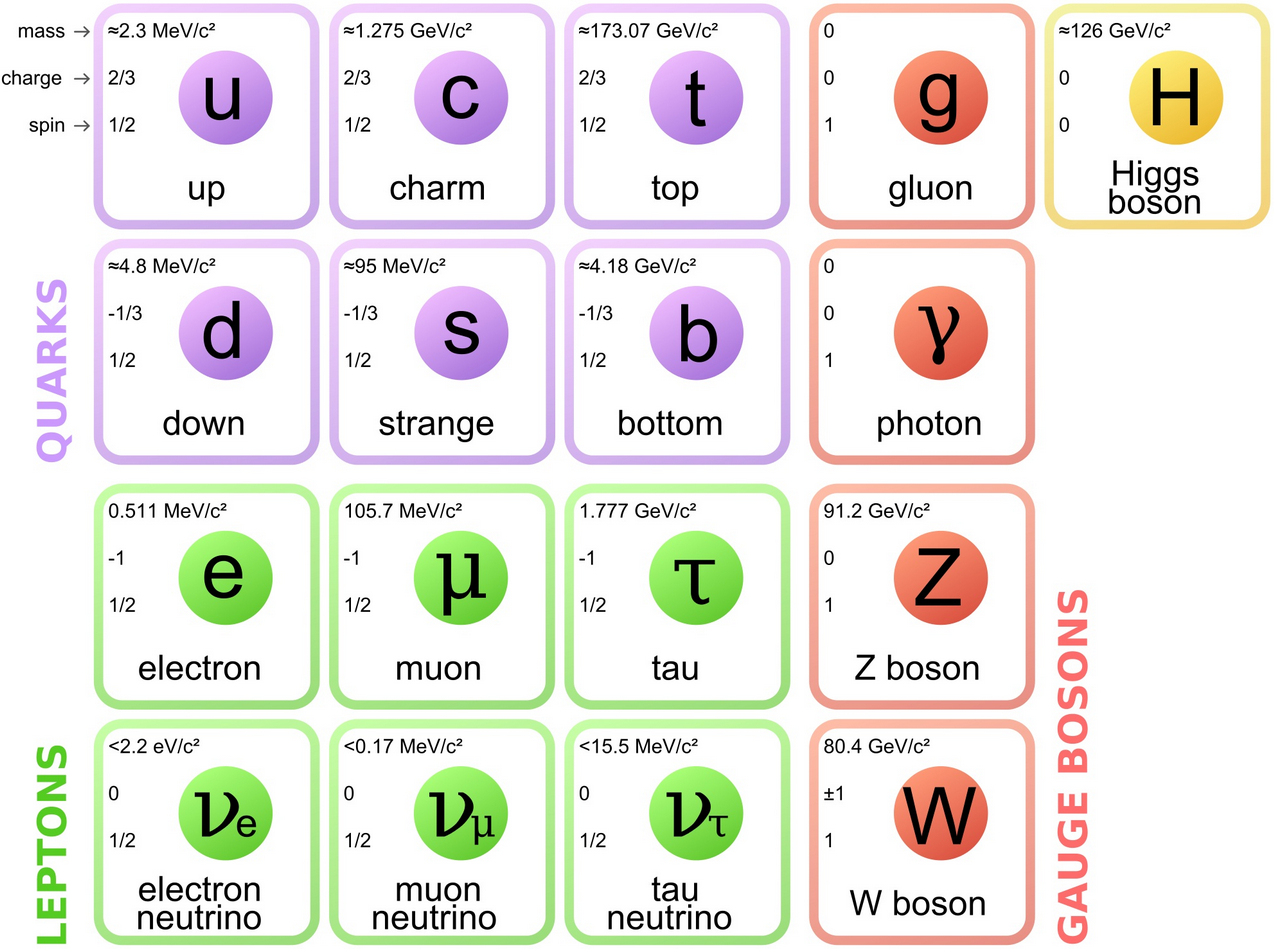
\includegraphics[width=0.8\textwidth]{standardModel.png}
\end{center}

With that out of the way, we'll continue our discussion of the fundamental forces, sans gravity.
\begin{itemize}
    \item Electromagnetic force.
    We're familiar with the associated potential function
    \[ V(r) = \frac{(Q_1 e)(Q_2 e)}{4\pi \epsilon_0 \hbar c} \frac{\hbar c}{r} = Q_1 Q_2 \left( \frac{e^2}{4\pi \epsilon_0 \hbar c} \right) \frac{\hbar c}{r}, \]
    where $q_i = Q_i q_e$.
    We'll also package the parenthetical into a dimensionless coupling constant $\alpha_\gamma$ to get
    \[ V(r) = Q_1 Q_2 \,\alpha_\gamma\, \frac{\hbar c}{r}. \]
    In summary we have $a_\gamma \simeq 1 / 137 \simeq 0.0073$, $m_\gamma = Q_\gamma = 0$, and an infinite range.

    \item Weak force.
    This more unfamiliar force is responsible for radioactive decay.
    Its potential takes a similar form, but this time there is a massive force carrier so we tack on an extra factor:
    \[ V(r) = Q_1^W Q_2^W \,\alpha_W\, \frac{\hbar c}{r} e^{-c m_W r / \hbar}. \]
    The exponential causes the force to essentially vanish for $r \sim \hbar / cm_W$, where the W and Z masses are each about 100 times bigger than that of a proton.
    The weak force has $\alpha_W \simeq 0.032$, and the charge is simply called ``weak charge''.

    \item Strong force.
    This force is chiefly responsible for holding nucleons together, but its effects spill out and build full nuclei, too.
    Its coupling strength is not constant due to self-interaction, but it tends to be around $\alpha_S \simeq 0.1$.
    The charge is called color, and it turns out that the gluon itself has color!
    (Self-interaction also leads to the strange observation that the strong force, to a point, gets stronger with distance and with decreasing energy.)
\end{itemize}
It turns out that quarks and gluons always get bound together into color-neutral states called mesons or baryons, together hadrons.
Mesons are comprised of a quark and an antiquark, while a baryon is comprised of three ordinary quarks.

Now, at high energies both matter and force carriers behave like these individual particles rather than waves.
Working with potentials becomes less useful, so we instead turn to computing probabilities of certain particle interactions taking place.
These probabilities are encoded in Feynman diagrams, which have an amount of mathematical complexity that is beyond the scope of this course; for now we'll focus on the surface level.

\parbox{0.66\textwidth}{
    \vspace{6pt}
    At right is an example of a Feynman diagram.
    There are few things to notice here.
    First is that the diagram is read from bottom to top; here we start with an electron, then a photon is produced, and we end with an electron.
    So this diagram represents the emission of a photon when an electron falls to a lower energy state!

    \vspace{6pt}
    Also, the arrowheads on the two electron lines have nothing to do with the passage of time or movement in space.
    Instead, the fact that they point in the same direction as time simply emphasizes that we are talking about electrons rather than positrons, whose arrows point against time.    
}\parbox{0.34\textwidth}{
    \quad\;
    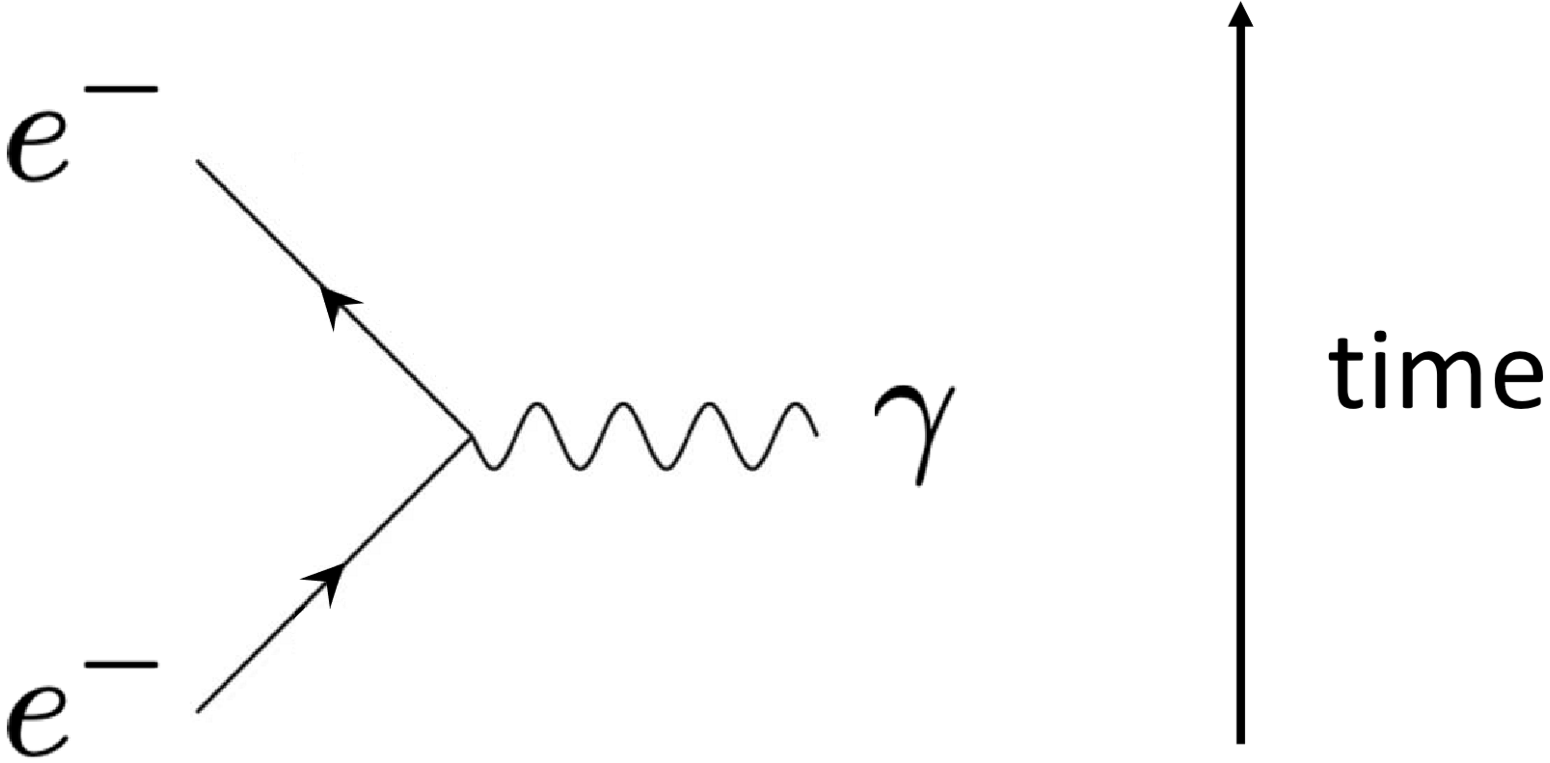
\includegraphics[width=0.3\textwidth]{feynmanEmission.png}
}

We can also use Feynman diagrams to represent unknown processes.
We write down the inputs to the processes, send them into a ``black box'' (however we decide to draw that), and get back some outputs.
Roughly speaking, each possibility for the contents of the black box is associated with a probability amplitude; we can add them, norm them, and square them to determine the probability of this arbitrary process occurring.

Most relevant to us right now, we can use Feynman diagrams to represent some key insights about the nature of the weak force.
First, the $W^\pm$ interactions are the only ones in the Standard Model that change the type of a particle---for example, an $e^-$ might interact with a $W^-$ to create an $\nu_e$.
Thus these bosons are the only force carriers that allow matter particles to decay!
For leptons, however, this comes with the caveat that the $W^\pm$ only couple charged leptons and neutrinos of the same generation, so we couldn't have an interaction involving $e^- \to \nu_\mu$, for example.

Speaking of neutrinos, their observations have been plagued by a puzzle that goes beyond the Standard Model---on Earth, we only observe a third of the predicted number of solar neutrinos!
This was a complex problem for a long time, but it turns out to have a simple solution: neutrinos cannot be in energy eigenstates.
Focusing just on the electron and muon neutrinos, consider two actual eigenstates $\psi_1, \psi_2$.
Then we have
\begin{align*}
    \psi_{\nu_e} &= (\cos \theta) \psi_1 + (\sin \theta) \psi_2 \\
    \psi_{\nu_\mu} &= (-\sin \theta) \psi_1 + (\cos \theta) \psi_2
\end{align*}
We can put these together to find the most general wave function:
\begin{align*}
    \Psi(t) &= (\cos \theta) e^{-iE_1 t / \hbar} \psi_1 + (\sin \theta) e^{-iE_2 t / \hbar} \psi_2 \\
    &= c_e(t) \psi_{\nu_e} + c_\mu(t) \psi_{\nu_\mu}
\end{align*}
As $\Psi(t)$ evolves, the probability associated with each term evolves too, and we come to the startling conclusion that neutrinos can change type as time passes!
This completely explains the perceived deficit in neutrinos.

\section{Compact Extra Dimensions}
Now we'll investigate one last problem: why is gravity so puny compared to the other fundamental forces?
One purely theoretical hypothesis is that its influence is being eaten up by some other spatial dimensions that we can't see.
Let's run with this and see where it goes!

Recall Gauss's law $\nabla \cdot \mbf{E} = \rho / \epsilon_0$, and how we can use it to derive Coulomb's law.
It turns out that there is an analog for gravitation: $\nabla \cdot \mbf{g} = -4\pi G \rho_m$, where $\rho_m$ is mass density.
Integrating over a volume $V$ gives
\[ \int_{\partial V} \mbf{g} \cdot d\mbf{A} = -4\pi Gm \implies \mbf{g} = -\frac{GM}{r^2} \hat r, \]
where the second statement comes from placing a point mass inside a radius-$r$ sphere.
If we generalize this process to (3 + $n$)-dimensional space we get
\[ \mbf{g} = -\frac{G_n M}{r^{2+n}} \hat r, \]
where $G_n$ is a generalized gravitational constant.

Now, suppose that these $n$ extra dimensions are compact with characteristic ``radius'' $R$.
To understand this, we might draw an analogy to a person and ant walking on a radius-$R$ tightrope
The walker can only experience forward-backward motion, but a creature as small as an ant would notice that it can walk all the way around the tightrope, effectively adding a new compact dimension to the picture.
See how, despite the existence of such dimensions, over long distances $r \gg R$ in the visible dimensions we recover the somewhat familiar
\[ g = -\frac{G_n M}{R^n r^2} \equiv \frac{G_N^\textrm{3D} M}{r^2}. \]
This is great, but gravity is fundamentally tied to relativity, which we know is incompatible with the Schrödinger equation.
What we need is a relativistic wave equation, and the Klein-Gordon equation does the trick:
\[ -\hbar^2 c^2 \nabla^2 \Psi + m^2 c^{4} \Psi = -\hbar^2 \frac{\partial^2 \Psi}{\partial t^2}. \]
Note that this equation has the dispersion relation $h \omega = \sqrt{\hbar^2 k^2 c^2 + m^2 c^{4}}$, as we'd hope based on our knowledge of special relativity.
Now, suppose we introduce a fourth compact coordinate $u$, so the Laplacian turns into
\[ \nabla^2 = \frac{\partial^2}{\partial x^2} + \frac{\partial^2}{\partial y^2} + \frac{\partial^2}{\partial z^2} + \frac{\partial^2}{\partial u^2}. \]
We'll rewrite the Klein-Gordon equation:
\[ \hbar^2 c^2 \left[ \frac{1}{c^2} \frac{\partial^2 \Psi}{\partial t^2} - \nabla^2 \Psi \right] + m^2 c^{4} \Psi = 0. \]
The solution looks like
\begin{align*}
    \Psi(x,y,z,u,t) &= e^{-iEt / \hbar} e^{i(k_xx + k_yy + k_zz + k_uu)} \\
    &= e^{-iEt / \hbar} e^{i(\mbf{k} \cdot \mbf{x} + k_uu)}.
\end{align*}
As a gut check, we could substitute this back into the equation to confirm that $\Psi$ obeys the expected energy-momentum relation.
Now we apply a boundary condition; specifically, $u$ is a compact dimension, so to keep our wave function single-valued we require that $\Psi(\mbf{x},u,t) = \Psi(\mbf{x},u + 2\pi R,t)$.
Substituting the solution we just found gives
\[ e^{ik_uu} = e^{ik_u (u + 2\pi R)} \implies k_u = \frac{n}{R}, \quad n \in \mathbb{Z}. \]
So the energy eigenfunctions and eigenvalues are still quantized here!
The squared eigenvalues are
\[ E_n^2 = \hbar^2 |\mbf{k}|^2 c^2 + \frac{\hbar^2 c^2 n^2}{R^2} + m^2 c^{4}. \]
In the rest frame of the particle, the first term vanishes and we get
\[ m_n = \sqrt{m^2 + \frac{\hbar^2 n^2}{R^2 c^2}}. \]
This is the apparent mass of the particle in three dimensions!
All this is a peek into the world of things like string theory, where predictions only work out for universes with more than three dimensions.

\end{document}
%<3
%<3
%<3